\begin{figure}[!h]
  \begin{center}
    \caption{Partition du plan par la droite $D\equiv -x+2y=0$ et deux demi-plans}%
    \label{sep:ill}
    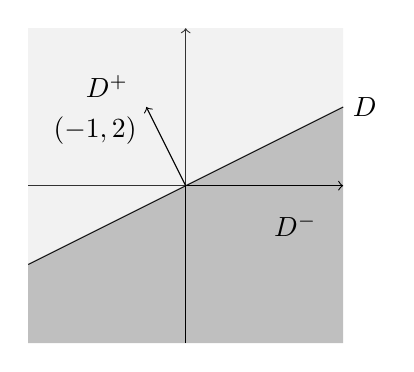
\begin{tikzpicture}
      \draw [->] (0, -2) -- (0, 2);
      \draw [->] (-2, 0) -- (2, 0);
      \draw (-2, -1) -- (2, 1) node[right] {$D$};
      \fill [black, nearly transparent] %
      (-2, -1) -- (2, 1) -- (2, -2) -- (-2, -2) -- cycle;
      \draw (1, -0.5) node[right] {$D^-$};
      \fill [black!20, nearly transparent] %
      (-2, -1) -- (2, 1) -- (2, 2) -- (-2, 2) -- cycle;
      \draw (-1, 1) node[above] {$D^+$};
      \draw [->] (0, 0) -- (-0.5, 1) node[below left] {$(-1, 2)$};
    \end{tikzpicture}
\end{center}
\end{figure}

%%% Local Variables:
%%% mode: latex
%%% TeX-master: "../rapportGp1"
%%% End:
